% Options for packages loaded elsewhere
\PassOptionsToPackage{unicode}{hyperref}
\PassOptionsToPackage{hyphens}{url}
%
\documentclass[
]{article}
\usepackage{amsmath,amssymb}
\usepackage{iftex}
\ifPDFTeX
  \usepackage[T1]{fontenc}
  \usepackage[utf8]{inputenc}
  \usepackage{textcomp} % provide euro and other symbols
\else % if luatex or xetex
  \usepackage{unicode-math} % this also loads fontspec
  \defaultfontfeatures{Scale=MatchLowercase}
  \defaultfontfeatures[\rmfamily]{Ligatures=TeX,Scale=1}
\fi
\usepackage{lmodern}
\ifPDFTeX\else
  % xetex/luatex font selection
\fi
% Use upquote if available, for straight quotes in verbatim environments
\IfFileExists{upquote.sty}{\usepackage{upquote}}{}
\IfFileExists{microtype.sty}{% use microtype if available
  \usepackage[]{microtype}
  \UseMicrotypeSet[protrusion]{basicmath} % disable protrusion for tt fonts
}{}
\makeatletter
\@ifundefined{KOMAClassName}{% if non-KOMA class
  \IfFileExists{parskip.sty}{%
    \usepackage{parskip}
  }{% else
    \setlength{\parindent}{0pt}
    \setlength{\parskip}{6pt plus 2pt minus 1pt}}
}{% if KOMA class
  \KOMAoptions{parskip=half}}
\makeatother
\usepackage{xcolor}
\usepackage[margin=1in]{geometry}
\usepackage{color}
\usepackage{fancyvrb}
\newcommand{\VerbBar}{|}
\newcommand{\VERB}{\Verb[commandchars=\\\{\}]}
\DefineVerbatimEnvironment{Highlighting}{Verbatim}{commandchars=\\\{\}}
% Add ',fontsize=\small' for more characters per line
\usepackage{framed}
\definecolor{shadecolor}{RGB}{248,248,248}
\newenvironment{Shaded}{\begin{snugshade}}{\end{snugshade}}
\newcommand{\AlertTok}[1]{\textcolor[rgb]{0.94,0.16,0.16}{#1}}
\newcommand{\AnnotationTok}[1]{\textcolor[rgb]{0.56,0.35,0.01}{\textbf{\textit{#1}}}}
\newcommand{\AttributeTok}[1]{\textcolor[rgb]{0.13,0.29,0.53}{#1}}
\newcommand{\BaseNTok}[1]{\textcolor[rgb]{0.00,0.00,0.81}{#1}}
\newcommand{\BuiltInTok}[1]{#1}
\newcommand{\CharTok}[1]{\textcolor[rgb]{0.31,0.60,0.02}{#1}}
\newcommand{\CommentTok}[1]{\textcolor[rgb]{0.56,0.35,0.01}{\textit{#1}}}
\newcommand{\CommentVarTok}[1]{\textcolor[rgb]{0.56,0.35,0.01}{\textbf{\textit{#1}}}}
\newcommand{\ConstantTok}[1]{\textcolor[rgb]{0.56,0.35,0.01}{#1}}
\newcommand{\ControlFlowTok}[1]{\textcolor[rgb]{0.13,0.29,0.53}{\textbf{#1}}}
\newcommand{\DataTypeTok}[1]{\textcolor[rgb]{0.13,0.29,0.53}{#1}}
\newcommand{\DecValTok}[1]{\textcolor[rgb]{0.00,0.00,0.81}{#1}}
\newcommand{\DocumentationTok}[1]{\textcolor[rgb]{0.56,0.35,0.01}{\textbf{\textit{#1}}}}
\newcommand{\ErrorTok}[1]{\textcolor[rgb]{0.64,0.00,0.00}{\textbf{#1}}}
\newcommand{\ExtensionTok}[1]{#1}
\newcommand{\FloatTok}[1]{\textcolor[rgb]{0.00,0.00,0.81}{#1}}
\newcommand{\FunctionTok}[1]{\textcolor[rgb]{0.13,0.29,0.53}{\textbf{#1}}}
\newcommand{\ImportTok}[1]{#1}
\newcommand{\InformationTok}[1]{\textcolor[rgb]{0.56,0.35,0.01}{\textbf{\textit{#1}}}}
\newcommand{\KeywordTok}[1]{\textcolor[rgb]{0.13,0.29,0.53}{\textbf{#1}}}
\newcommand{\NormalTok}[1]{#1}
\newcommand{\OperatorTok}[1]{\textcolor[rgb]{0.81,0.36,0.00}{\textbf{#1}}}
\newcommand{\OtherTok}[1]{\textcolor[rgb]{0.56,0.35,0.01}{#1}}
\newcommand{\PreprocessorTok}[1]{\textcolor[rgb]{0.56,0.35,0.01}{\textit{#1}}}
\newcommand{\RegionMarkerTok}[1]{#1}
\newcommand{\SpecialCharTok}[1]{\textcolor[rgb]{0.81,0.36,0.00}{\textbf{#1}}}
\newcommand{\SpecialStringTok}[1]{\textcolor[rgb]{0.31,0.60,0.02}{#1}}
\newcommand{\StringTok}[1]{\textcolor[rgb]{0.31,0.60,0.02}{#1}}
\newcommand{\VariableTok}[1]{\textcolor[rgb]{0.00,0.00,0.00}{#1}}
\newcommand{\VerbatimStringTok}[1]{\textcolor[rgb]{0.31,0.60,0.02}{#1}}
\newcommand{\WarningTok}[1]{\textcolor[rgb]{0.56,0.35,0.01}{\textbf{\textit{#1}}}}
\usepackage{graphicx}
\makeatletter
\def\maxwidth{\ifdim\Gin@nat@width>\linewidth\linewidth\else\Gin@nat@width\fi}
\def\maxheight{\ifdim\Gin@nat@height>\textheight\textheight\else\Gin@nat@height\fi}
\makeatother
% Scale images if necessary, so that they will not overflow the page
% margins by default, and it is still possible to overwrite the defaults
% using explicit options in \includegraphics[width, height, ...]{}
\setkeys{Gin}{width=\maxwidth,height=\maxheight,keepaspectratio}
% Set default figure placement to htbp
\makeatletter
\def\fps@figure{htbp}
\makeatother
\setlength{\emergencystretch}{3em} % prevent overfull lines
\providecommand{\tightlist}{%
  \setlength{\itemsep}{0pt}\setlength{\parskip}{0pt}}
\setcounter{secnumdepth}{-\maxdimen} % remove section numbering
\ifLuaTeX
  \usepackage{selnolig}  % disable illegal ligatures
\fi
\IfFileExists{bookmark.sty}{\usepackage{bookmark}}{\usepackage{hyperref}}
\IfFileExists{xurl.sty}{\usepackage{xurl}}{} % add URL line breaks if available
\urlstyle{same}
\hypersetup{
  pdftitle={Minería de Texto},
  pdfauthor={Iván Mendivelso},
  hidelinks,
  pdfcreator={LaTeX via pandoc}}

\title{Minería de Texto}
\author{Iván Mendivelso}
\date{2023-11-20}

\begin{document}
\maketitle

\hypertarget{paquetes-para-esta-sesiuxf3n}{%
\subsection{Paquetes para esta
sesión}\label{paquetes-para-esta-sesiuxf3n}}

\begin{Shaded}
\begin{Highlighting}[]
\FunctionTok{install.packages}\NormalTok{(}\StringTok{"tm"}\NormalTok{)}
\FunctionTok{install.packages}\NormalTok{(}\StringTok{"pdftools"}\NormalTok{)}
\FunctionTok{install.packages}\NormalTok{(}\StringTok{"stopwords"}\NormalTok{)}
\FunctionTok{install.packages}\NormalTok{(}\StringTok{"wordcloud"}\NormalTok{)}
\FunctionTok{install.packages}\NormalTok{(}\StringTok{"quanteda"}\NormalTok{)}
\end{Highlighting}
\end{Shaded}

\begin{Shaded}
\begin{Highlighting}[]
\FunctionTok{library}\NormalTok{(tidyverse)}
\FunctionTok{library}\NormalTok{(tm)}
\FunctionTok{library}\NormalTok{(pdftools)}
\FunctionTok{library}\NormalTok{(stopwords)}
\FunctionTok{library}\NormalTok{(wordcloud)}
\FunctionTok{library}\NormalTok{(quanteda)}
\end{Highlighting}
\end{Shaded}

\hypertarget{preliminares}{%
\subsection{Preliminares}\label{preliminares}}

El análisis de datos textuales, también conocido como minería de texto o
\emph{text mining}, permite extraer información valiosa y conocimientos
de inmensas cantidades de texto no estructurado. Esta área
interdisciplinaria combina técnicas de la lingüística computacional, la
estadística, y la inteligencia artificial para procesar, analizar y
comprender el lenguaje natural, abriendo puertas a un mundo de
posibilidades en diversos campos, desde el marketing hasta la salud. En
tiempos recientes, el avance de los modelos de lenguaje de aprendizaje
profundo, especialmente los Grandes Modelos de Lenguaje (LLM, por sus
siglas en inglés), ha revolucionado aún más este campo. Estos modelos,
entrenados en gigantescos corpus de texto, no solo entienden y generan
lenguaje natural con una precisión asombrosa, sino que también son
capaces de captar matices y contextos complejos, ofreciendo
interpretaciones y análisis más ricos y profundos.

Los LLM, como ChatGPT de OpenAI, Bard de Google, entre otros, han
ampliado significativamente el alcance y la profundidad del análisis de
texto. No se limitan a tareas tradicionales como la clasificación de
texto, la extracción de entidades o el análisis de sentimientos; pueden
realizar tareas más sofisticadas como la generación de resúmenes, la
creación de contenido, la traducción automática, y hasta la programación
basada en descripciones en lenguaje natural. Esta capacidad para manejar
tareas complejas y diversas ha llevado a que los LLM se integren en una
variedad de aplicaciones, desde asistentes virtuales hasta herramientas
avanzadas de análisis de datos.

Sin embargo, a pesar de sus capacidades, los LLM presentan desafíos
importantes, como la necesidad de grandes recursos computacionales y la
gestión de sesgos inherentes a los datos de entrenamiento. A medida que
el tiempo avanza y estos modelos se desarrollan, es crucial abordar
estos desafíos, garantizando que el análisis de texto siga siendo una
herramienta poderosa y ética para descubrir \emph{insights} entre
grandes cantidades de texto sin estructurar.

El desarrollo de los LLM es complejo y está por fuera del alcance de
esta sesión de clase, puesto que requiere un alto acervo teórico y
capacidades computacionales (si se tiene interés en este tema, se
sugiere buscar en Google el artículo ``\emph{Attention is All You
Need}''), por lo que aquí se tratarán las aplicaciones tradicionales del
análisis de datos textuales como son la creación de un corpus de texto,
la tokenización, el análisis de frecuencias, la visualización de datos y
generación de digramas y trigramas.

\begin{Shaded}
\begin{Highlighting}[]
\NormalTok{textos }\OtherTok{\textless{}{-}} \FunctionTok{c}\NormalTok{(}\StringTok{"Soy un dios en mi pueblo y en mi valle."}\NormalTok{, }
            \StringTok{"No porque me adoren, sino porque yo lo hago."}\NormalTok{, }
            \StringTok{"Porque me inclino ante quien me regala"}\NormalTok{,}
            \StringTok{"Unas granadillas o una sonrisa de su heredad..."}\NormalTok{)}
\FunctionTok{class}\NormalTok{(textos)}
\end{Highlighting}
\end{Shaded}

\begin{verbatim}
## [1] "character"
\end{verbatim}

\begin{Shaded}
\begin{Highlighting}[]
\NormalTok{textos}
\end{Highlighting}
\end{Shaded}

\begin{verbatim}
## [1] "Soy un dios en mi pueblo y en mi valle."        
## [2] "No porque me adoren, sino porque yo lo hago."   
## [3] "Porque me inclino ante quien me regala"         
## [4] "Unas granadillas o una sonrisa de su heredad..."
\end{verbatim}

\hypertarget{conceptos-importantes}{%
\subsection{Conceptos importantes}\label{conceptos-importantes}}

\hypertarget{corpus}{%
\subsection{Corpus}\label{corpus}}

Un corpus de texto es una colección grande y estructurada de textos que
se utiliza para el análisis lingüístico y el procesamiento del lenguaje
natural (PLN). En R, un corpus puede ser manipulado y analizado
utilizando diversos paquetes y funciones especializadas.

Un corpus en R generalmente se crea importando datos de texto desde
diversas fuentes como archivos de texto, PDFs, o incluso directamente
desde la web. El paquete \texttt{tm} (Text Mining) es uno de los más
populares para trabajar con corpus de texto.

Un corpus puede ser una colección simple de textos o una estructura más
compleja que incluye metadatos sobre cada texto, como autor, fecha,
fuente, etc. Esto permite análisis más sofisticados y específicos.

Con el corpus listo, se pueden realizar diversos análisis como la
frecuencia de palabras, la co-ocurrencia de términos, el análisis de
sentimientos, la clasificación de textos, entre otros. Estos análisis
ayudan a extraer \emph{insights} y patrones de los datos de texto.

\begin{Shaded}
\begin{Highlighting}[]
\NormalTok{vector\_fuente }\OtherTok{\textless{}{-}} \FunctionTok{VectorSource}\NormalTok{(textos)}

\NormalTok{corpus }\OtherTok{\textless{}{-}} \FunctionTok{Corpus}\NormalTok{(vector\_fuente)}

\FunctionTok{class}\NormalTok{(corpus)}
\end{Highlighting}
\end{Shaded}

\begin{verbatim}
## [1] "SimpleCorpus" "Corpus"
\end{verbatim}

\begin{Shaded}
\begin{Highlighting}[]
\FunctionTok{inspect}\NormalTok{(corpus) }
\end{Highlighting}
\end{Shaded}

\begin{verbatim}
## <<SimpleCorpus>>
## Metadata:  corpus specific: 1, document level (indexed): 0
## Content:  documents: 4
## 
## [1] Soy un dios en mi pueblo y en mi valle.        
## [2] No porque me adoren, sino porque yo lo hago.   
## [3] Porque me inclino ante quien me regala         
## [4] Unas granadillas o una sonrisa de su heredad...
\end{verbatim}

\hypertarget{term-document-matrix}{%
\subsection{\texorpdfstring{\emph{Term-Document
Matrix}}{Term-Document Matrix}}\label{term-document-matrix}}

La \emph{Term-Document Matrix} es una matriz donde cada fila representa
un término único (generalmente una palabra) y cada columna representa un
documento del corpus. Los elementos de la matriz indican la frecuencia
de cada término en cada documento.

\begin{Shaded}
\begin{Highlighting}[]
\NormalTok{tdm }\OtherTok{\textless{}{-}} \FunctionTok{TermDocumentMatrix}\NormalTok{(corpus)}
\NormalTok{tdm\_matrix }\OtherTok{\textless{}{-}} \FunctionTok{as.matrix}\NormalTok{(tdm)}
\NormalTok{tdm\_matrix }\SpecialCharTok{\%\textgreater{}\%} \FunctionTok{head}\NormalTok{()}
\end{Highlighting}
\end{Shaded}

\begin{verbatim}
##          Docs
## Terms     1 2 3 4
##   dios    1 0 0 0
##   pueblo  1 0 0 0
##   soy     1 0 0 0
##   valle.  1 0 0 0
##   adoren, 0 1 0 0
##   hago.   0 1 0 0
\end{verbatim}

\hypertarget{tokenizaciuxf3n}{%
\subsection{Tokenización}\label{tokenizaciuxf3n}}

La tokenización es el proceso de dividir un texto o una cadena de
caracteres en unidades más pequeñas llamadas ``tokens''. Un token, en
este contexto, suele ser una palabra, aunque también puede ser un
símbolo, un número, o cualquier otro elemento significativo en el texto.

La tokenización es a menudo el primer paso en el análisis de texto y
PLN. Al dividir el texto en tokens, se facilita la realización de tareas
como el conteo de frecuencia de palabras, la identificación de patrones
de lenguaje, el análisis de sentimientos, la clasificación de textos,
entre otros.

Este proceso ayuda a estandarizar el texto para el análisis posterior.
Por ejemplo, al dividir el texto en palabras individuales, se pueden
aplicar operaciones como convertir todo el texto a minúsculas, eliminar
la puntuación, y realizar la lematización o el \emph{stemming} (reducir
las palabras a su raíz o forma base).

La tokenización es crucial para manejar la diversidad en el uso del
lenguaje. Diferentes idiomas y contextos (como el lenguaje coloquial,
técnico, o literario) pueden requerir diferentes enfoques de
tokenización.

\begin{Shaded}
\begin{Highlighting}[]
\NormalTok{matriz }\OtherTok{\textless{}{-}} \FunctionTok{as.matrix}\NormalTok{(tdm)}

\NormalTok{palabras\_frecuencia }\OtherTok{\textless{}{-}} \FunctionTok{rowSums}\NormalTok{(matriz)}

\NormalTok{palabras\_frecuencia }\OtherTok{\textless{}{-}} \FunctionTok{sort}\NormalTok{(palabras\_frecuencia, }\AttributeTok{decreasing =} \ConstantTok{TRUE}\NormalTok{)}

\NormalTok{palabras\_frecuencia}
\end{Highlighting}
\end{Shaded}

\begin{verbatim}
##      porque        dios      pueblo         soy      valle.     adoren, 
##           3           1           1           1           1           1 
##       hago.        sino        ante     inclino       quien      regala 
##           1           1           1           1           1           1 
## granadillas  heredad...     sonrisa         una        unas 
##           1           1           1           1           1
\end{verbatim}

\hypertarget{preprocesamiento}{%
\subsection{Preprocesamiento}\label{preprocesamiento}}

El preprocesamiento de un corpus de texto es un conjunto de pasos
diseñados para limpiar y estandarizar los datos de texto antes de
realizar análisis más complejos. Los pasos que normalmente se siguen
para realizar el preprocesamiento de un corpus de texto son:

\begin{itemize}
\tightlist
\item
  Convertir a minúsculas: Hacer que todo el texto sea minúscula para que
  el análisis no sea sensible a las mayúsculas.
\end{itemize}

\begin{Shaded}
\begin{Highlighting}[]
\NormalTok{corpus }\OtherTok{\textless{}{-}} \FunctionTok{tm\_map}\NormalTok{(corpus, }\FunctionTok{content\_transformer}\NormalTok{(tolower))}
\end{Highlighting}
\end{Shaded}

\begin{itemize}
\tightlist
\item
  Eliminar puntuación: Quitar los signos de puntuación, ya que
  generalmente no son necesarios para muchos tipos de análisis.
\end{itemize}

\begin{Shaded}
\begin{Highlighting}[]
\NormalTok{corpus }\OtherTok{\textless{}{-}} \FunctionTok{tm\_map}\NormalTok{(corpus, removePunctuation)}
\end{Highlighting}
\end{Shaded}

\begin{itemize}
\tightlist
\item
  Eliminar números: Opcionalmente es posible quitar los números si no
  son relevantes para el análisis.
\end{itemize}

\begin{Shaded}
\begin{Highlighting}[]
\NormalTok{corpus }\OtherTok{\textless{}{-}} \FunctionTok{tm\_map}\NormalTok{(corpus, removeNumbers)}
\end{Highlighting}
\end{Shaded}

\begin{itemize}
\tightlist
\item
  Eliminar espacios en blanco extra: Limpiar espacios extra, como los
  espacios al principio y al final del texto, o múltiples espacios
  seguidos.
\end{itemize}

\begin{Shaded}
\begin{Highlighting}[]
\NormalTok{corpus }\OtherTok{\textless{}{-}} \FunctionTok{tm\_map}\NormalTok{(corpus, stripWhitespace)}
\end{Highlighting}
\end{Shaded}

\begin{itemize}
\tightlist
\item
  Eliminar \emph{stopwords}: Quitar palabras comunes que generalmente no
  aportan mucho significado al texto, como ``el'', ``la'', ``y'', etc.
\end{itemize}

\begin{Shaded}
\begin{Highlighting}[]
\NormalTok{corpus }\OtherTok{\textless{}{-}} \FunctionTok{tm\_map}\NormalTok{(corpus, removeWords, }\FunctionTok{stopwords}\NormalTok{(}\StringTok{"spanish"}\NormalTok{))}
\end{Highlighting}
\end{Shaded}

Las funciones mostradas como ejemplos en los anteriores \emph{script}
pertenecen a la biblioteca para análisis de texto \texttt{tm}.

\hypertarget{biblioteca-tm}{%
\subsection{\texorpdfstring{Biblioteca
\texttt{tm}}{Biblioteca tm}}\label{biblioteca-tm}}

El paquete \texttt{tm}, que significa ``Text Mining'', es uno de los
paquetes más prominentes y utilizados en R para el análisis de texto y
la minería de datos textuales. Diseñado para facilitar el manejo,
procesamiento y análisis de grandes conjuntos de datos textuales,
\texttt{tm} proporciona un marco de trabajo integral y flexible para
todo tipo de análisis de texto en R.

\texttt{tm} permite importar datos de texto desde varias fuentes, como
archivos de texto plano, archivos JSON, XML, y otros formatos. Esto hace
que sea fácil trabajar con una amplia gama de conjuntos de datos
textuales.

\hypertarget{ejemplo}{%
\subsubsection{Ejemplo}\label{ejemplo}}

\begin{Shaded}
\begin{Highlighting}[]
\NormalTok{ruta }\OtherTok{\textless{}{-}} \StringTok{\textquotesingle{}C:/Users/Ivan Mendivelso/OneDrive {-} OVERLAP INTERNACIONAL S.A/Documentos/GitHub/Cursos\_Overlap/titanic.csv\textquotesingle{}}
\NormalTok{datos }\OtherTok{\textless{}{-}} \FunctionTok{read.csv2}\NormalTok{(ruta)}
\FunctionTok{glimpse}\NormalTok{(datos)}
\end{Highlighting}
\end{Shaded}

\begin{verbatim}
## Rows: 1,309
## Columns: 12
## $ PassengerId <int> 1, 2, 3, 4, 5, 6, 7, 8, 9, 10, 11, 12, 13, 14, 15, 16, 17,~
## $ Survived    <int> 0, 1, 1, 1, 0, 0, 0, 0, 1, 1, 1, 1, 0, 0, 0, 1, 0, 1, 0, 1~
## $ Pclass      <int> 3, 1, 3, 1, 3, 3, 1, 3, 3, 2, 3, 1, 3, 3, 3, 2, 3, 2, 3, 3~
## $ Name        <chr> "Braund, Mr. Owen Harris", "Cumings, Mrs. John Bradley (Fl~
## $ Sex         <chr> "male", "female", "female", "female", "male", "male", "mal~
## $ Age         <dbl> 22, 38, 26, 35, 35, NA, 54, 2, 27, 14, 4, 58, 20, 39, 14, ~
## $ SibSp       <int> 1, 1, 0, 1, 0, 0, 0, 3, 0, 1, 1, 0, 0, 1, 0, 0, 4, 0, 1, 0~
## $ Parch       <int> 0, 0, 0, 0, 0, 0, 0, 1, 2, 0, 1, 0, 0, 5, 0, 0, 1, 0, 0, 0~
## $ Ticket      <chr> "A/5 21171", "PC 17599", "STON/O2. 3101282", "113803", "37~
## $ Fare        <dbl> 7.2500, 71.2833, 7.9250, 53.1000, 8.0500, 8.4583, 51.8625,~
## $ Cabin       <chr> NA, "C85", NA, "C123", NA, NA, "E46", NA, NA, NA, "G6", "C~
## $ Embarked    <chr> "S", "C", "S", "S", "S", "Q", "S", "S", "S", "C", "S", "S"~
\end{verbatim}

\begin{Shaded}
\begin{Highlighting}[]
\NormalTok{nombres }\OtherTok{\textless{}{-}}\NormalTok{ datos}\SpecialCharTok{$}\NormalTok{Name}
\NormalTok{vector\_fuente }\OtherTok{\textless{}{-}} \FunctionTok{VectorSource}\NormalTok{(nombres)}
\NormalTok{corpus\_nombres }\OtherTok{\textless{}{-}} \FunctionTok{Corpus}\NormalTok{(vector\_fuente)}
\end{Highlighting}
\end{Shaded}

\begin{Shaded}
\begin{Highlighting}[]
\FunctionTok{inspect}\NormalTok{(corpus\_nombres)}
\end{Highlighting}
\end{Shaded}

\begin{Shaded}
\begin{Highlighting}[]
\NormalTok{corpus\_nombres }\OtherTok{\textless{}{-}} \FunctionTok{tm\_map}\NormalTok{(corpus\_nombres, }\FunctionTok{content\_transformer}\NormalTok{(tolower))}

\NormalTok{corpus\_nombres }\OtherTok{\textless{}{-}} \FunctionTok{tm\_map}\NormalTok{(corpus\_nombres, removePunctuation)}

\NormalTok{corpus\_nombres }\OtherTok{\textless{}{-}} \FunctionTok{tm\_map}\NormalTok{(corpus\_nombres, removeNumbers)}

\NormalTok{tdm }\OtherTok{\textless{}{-}} \FunctionTok{TermDocumentMatrix}\NormalTok{(corpus\_nombres)}
\NormalTok{m }\OtherTok{\textless{}{-}} \FunctionTok{as.matrix}\NormalTok{(tdm)}
\NormalTok{word\_freqs }\OtherTok{\textless{}{-}} \FunctionTok{sort}\NormalTok{(}\FunctionTok{rowSums}\NormalTok{(m), }\AttributeTok{decreasing =} \ConstantTok{TRUE}\NormalTok{)}
\FunctionTok{head}\NormalTok{(word\_freqs)}
\end{Highlighting}
\end{Shaded}

\begin{verbatim}
##    miss     mrs william    john  master   henry 
##     260     201      87      72      61      49
\end{verbatim}

\hypertarget{stopwords}{%
\subsection{Stopwords}\label{stopwords}}

\begin{Shaded}
\begin{Highlighting}[]
\NormalTok{stopwords\_en }\OtherTok{\textless{}{-}} \FunctionTok{stopwords}\NormalTok{(}\StringTok{"en"}\NormalTok{)}
\end{Highlighting}
\end{Shaded}

\begin{Shaded}
\begin{Highlighting}[]
\NormalTok{corpus\_nombres }\OtherTok{\textless{}{-}} \FunctionTok{tm\_map}\NormalTok{(corpus\_nombres, removeWords, stopwords\_en)}

\NormalTok{tdm }\OtherTok{\textless{}{-}} \FunctionTok{TermDocumentMatrix}\NormalTok{(corpus\_nombres)}

\NormalTok{m }\OtherTok{\textless{}{-}} \FunctionTok{as.matrix}\NormalTok{(tdm)}

\NormalTok{word\_freqs }\OtherTok{\textless{}{-}} \FunctionTok{sort}\NormalTok{(}\FunctionTok{rowSums}\NormalTok{(m), }\AttributeTok{decreasing =} \ConstantTok{TRUE}\NormalTok{)}

\FunctionTok{head}\NormalTok{(word\_freqs)}
\end{Highlighting}
\end{Shaded}

\begin{verbatim}
##    miss     mrs william    john  master   henry 
##     260     201      87      72      61      49
\end{verbatim}

\hypertarget{visualizaciuxf3n-de-datos}{%
\subsection{Visualización de Datos}\label{visualizaciuxf3n-de-datos}}

R ofrece potentes herramientas de visualización como \texttt{ggplot2} y
\texttt{wordcloud} que se pueden usar para representar los resultados
del análisis de texto, facilitando la interpretación y presentación de
los datos.

\hypertarget{ejercicio-con-pdf}{%
\subsection{Ejercicio con PDF}\label{ejercicio-con-pdf}}

Seleccione un texto en formato PDF para aplicar los conceptos vistos
hasta el momento. Use la función \texttt{pdf\_text()} del paquete
\texttt{pdftools} para leer el documento. Luego realice los
correspondientes procedimientos para aplicar los métodos vistos.

\begin{verbatim}
##   que   del   los   las   una funes 
##   235    83    79    64    61    59
\end{verbatim}

\begin{verbatim}
##     funes nietzsche  historia   memoria    borges         “ 
##        59        59        47        34        32        27
\end{verbatim}

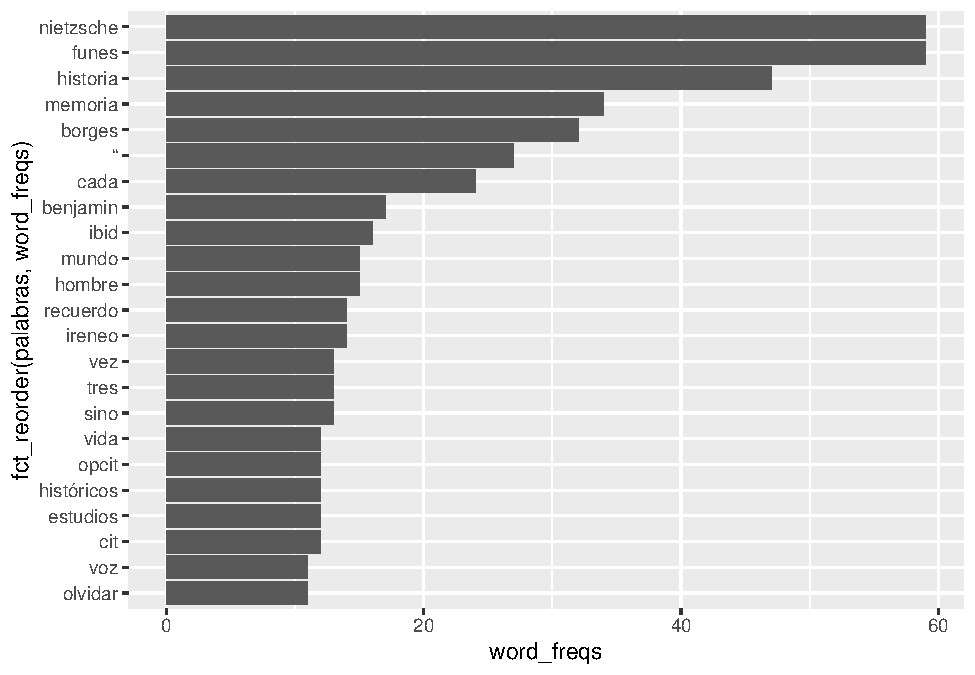
\includegraphics{Mineria_de_Texto_files/figure-latex/unnamed-chunk-22-1.pdf}

\hypertarget{wordclouds}{%
\subsubsection{Wordclouds}\label{wordclouds}}

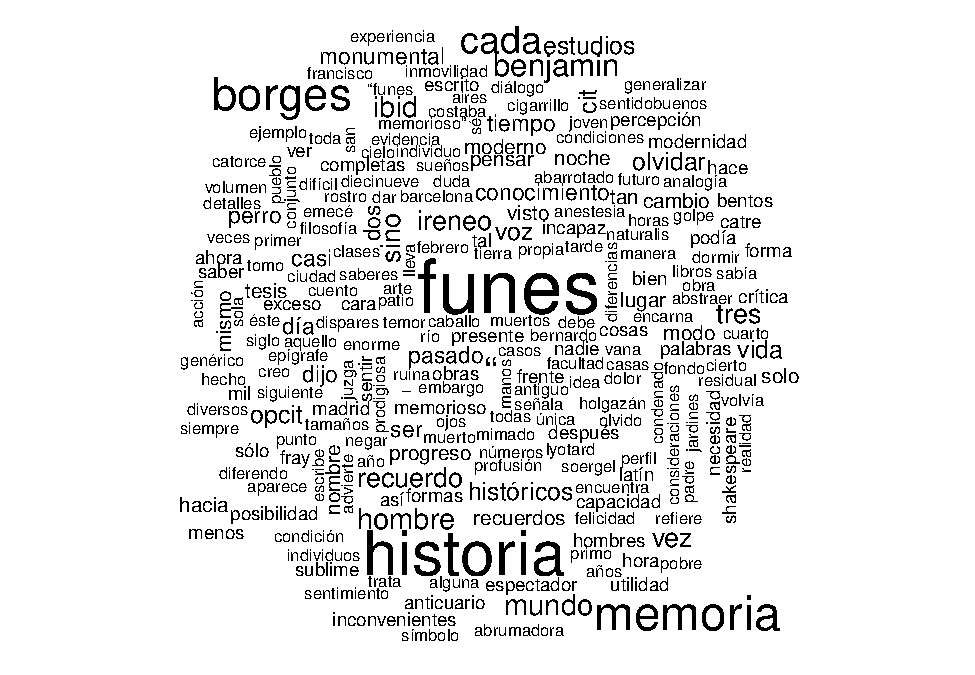
\includegraphics{Mineria_de_Texto_files/figure-latex/unnamed-chunk-23-1.pdf}

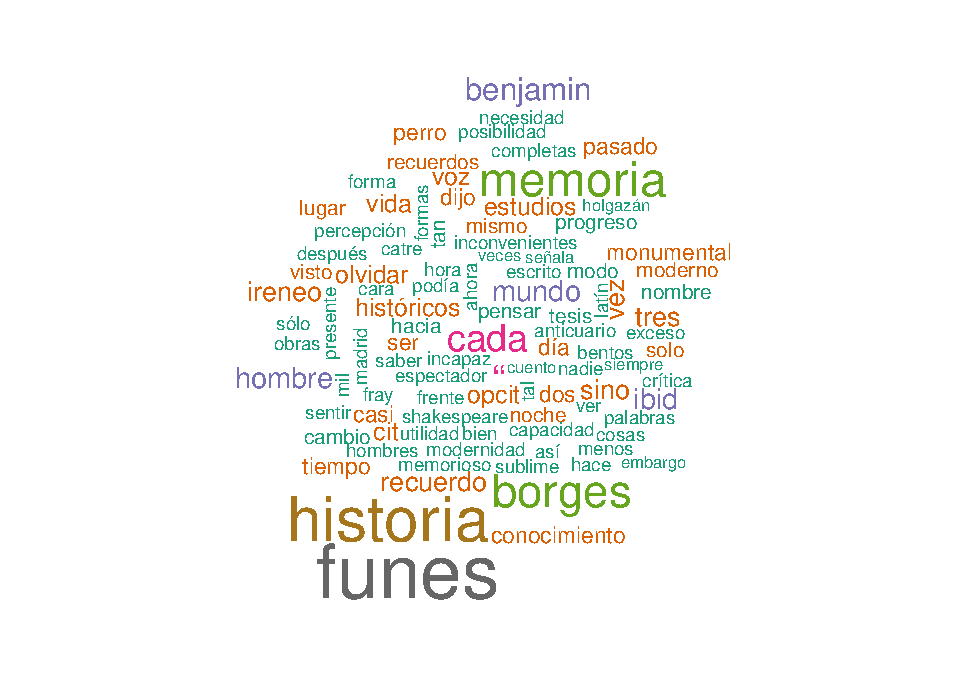
\includegraphics{Mineria_de_Texto_files/figure-latex/unnamed-chunk-24-1.pdf}

\hypertarget{digramas-y-trigramas}{%
\subsection{Digramas y trigramas}\label{digramas-y-trigramas}}

Los digramas y trigramas son conceptos fundamentales en el procesamiento
del lenguaje natural y el análisis de texto. Forman parte de los
n-gramas, que son secuencias contiguas de n elementos (o unidades)
extraídos de un texto.

\begin{Shaded}
\begin{Highlighting}[]
\NormalTok{texto }\OtherTok{\textless{}{-}} \FunctionTok{sapply}\NormalTok{(corpus\_texto, as.character)}

\NormalTok{corpus\_quanteda }\OtherTok{\textless{}{-}} \FunctionTok{corpus}\NormalTok{(texto)}

\NormalTok{tokens\_quanteda }\OtherTok{\textless{}{-}} \FunctionTok{tokens}\NormalTok{(corpus\_quanteda, }\AttributeTok{what =} \StringTok{"word"}\NormalTok{)}

\NormalTok{tokens\_digramas }\OtherTok{\textless{}{-}} \FunctionTok{tokens\_ngrams}\NormalTok{(tokens\_quanteda, }\AttributeTok{n =} \DecValTok{2}\NormalTok{)}
\NormalTok{tokens\_trigrams }\OtherTok{\textless{}{-}} \FunctionTok{tokens\_ngrams}\NormalTok{(tokens\_quanteda, }\AttributeTok{n =} \DecValTok{3}\NormalTok{)}

\NormalTok{dfm\_digramas }\OtherTok{\textless{}{-}} \FunctionTok{dfm}\NormalTok{(tokens\_digramas)}
\NormalTok{dfm\_trigrams }\OtherTok{\textless{}{-}} \FunctionTok{dfm}\NormalTok{(tokens\_trigrams)}
\end{Highlighting}
\end{Shaded}

\begin{Shaded}
\begin{Highlighting}[]
\NormalTok{top\_digramas }\OtherTok{\textless{}{-}} \FunctionTok{topfeatures}\NormalTok{(dfm\_digramas, }\DecValTok{10}\NormalTok{) }

\NormalTok{data\_digramas }\OtherTok{\textless{}{-}} \FunctionTok{data.frame}\NormalTok{(}\AttributeTok{ngram =} \FunctionTok{names}\NormalTok{(top\_digramas), }\AttributeTok{frequency =}\NormalTok{ top\_digramas)}

\FunctionTok{ggplot}\NormalTok{(data\_digramas, }\FunctionTok{aes}\NormalTok{(}\AttributeTok{x =} \FunctionTok{reorder}\NormalTok{(ngram, frequency), }\AttributeTok{y =}\NormalTok{ frequency)) }\SpecialCharTok{+}
    \FunctionTok{geom\_bar}\NormalTok{(}\AttributeTok{stat =} \StringTok{"identity"}\NormalTok{) }\SpecialCharTok{+}
    \FunctionTok{coord\_flip}\NormalTok{() }\SpecialCharTok{+}
    \FunctionTok{xlab}\NormalTok{(}\StringTok{"Digrama"}\NormalTok{) }\SpecialCharTok{+}
    \FunctionTok{ylab}\NormalTok{(}\StringTok{"Frecuencia"}\NormalTok{)}
\end{Highlighting}
\end{Shaded}

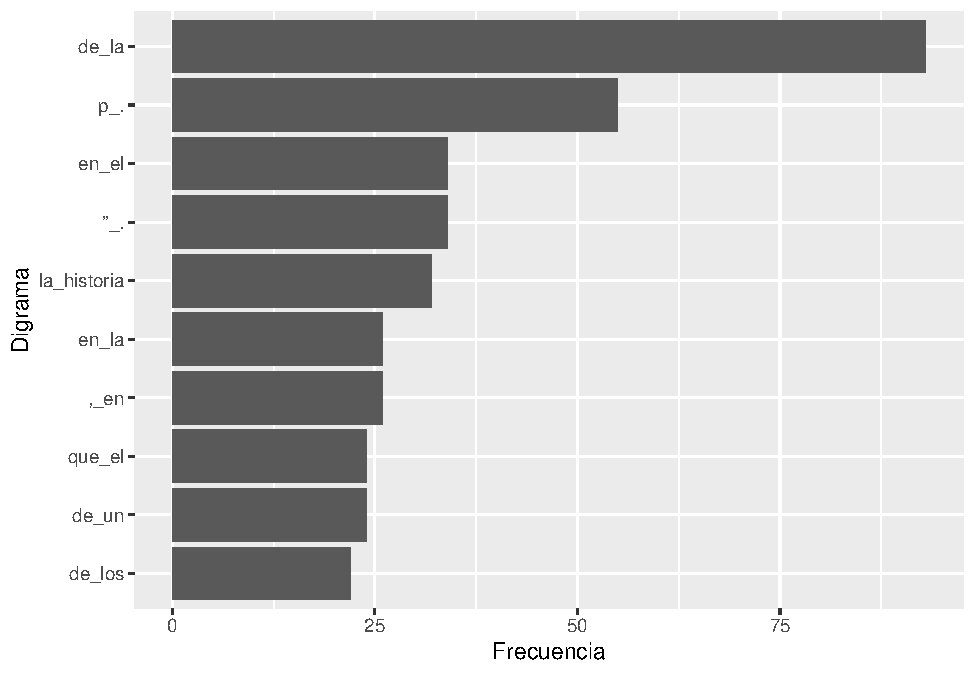
\includegraphics{Mineria_de_Texto_files/figure-latex/unnamed-chunk-26-1.pdf}

Elimine las \emph{stopwords} y realice de nuevo los digramas y
trigramas.

\end{document}
